\documentclass[a4paper, 12pt]{report}		% general format
\usepackage{multicol}
%%%% Charset
\usepackage{cmap}							% make PDF files searchable and copyable
\usepackage{bm}
\usepackage{pdfpages}
\usepackage[utf8x]{inputenc} 				% accept different input encodings
\usepackage[english,russian]{babel}   %% загружает пакет многоязыковой вёрстки
%\usepackage{fontspec}      %% подготавливает загрузку шрифтов Open Type, True Type и др.
%\defaultfontfeatures{Ligatures={TeX},Renderer=Basic}  %% свойства шрифтов по умолчанию
%\setmainfont[Ligatures={TeX,Historic}]{Roboto-Light} %% задаёт основной шрифт документа
%\setsansfont{Roboto-Light}  
\usepackage{float}
%%%% Graphics
%\usepackage[dvipsnames]{xcolor}			% driver-independent color extensions
\usepackage{graphicx}						% enhanced support for graphics
\usepackage{wrapfig}						% produces figures which text can flow around

%%%% Math
\usepackage{amsmath}						% American Mathematical Society (AMS) math facilities
\usepackage{amsfonts}						% fonts from the AMS
\usepackage{amssymb}						% additional math symbols

%%%% Typograpy (don't forget about cm-super)
\usepackage{microtype}						% subliminal refinements towards typographical perfection
\linespread{1.0}							% line spacing
\usepackage[mag=1000, left=2.0cm, right=1.5cm, top=2cm, bottom=2cm, headsep=0.7cm, footskip=1cm]{geometry}
\setlength{\parindent}{0pt}					% we don't want any paragraph indentation
\usepackage{parskip}						% some distance between paragraphs

%%%% Tables
\usepackage{tabularx}						% tables with variable width columns
\usepackage{multirow}						% for tabularx
\usepackage{hhline}							% for tabularx
\usepackage{tabu}
\usepackage{longtable}

%%%% Graph
\usepackage{tikz}							% package for creating graphics programmatically
\usetikzlibrary{arrows}						% edges for tikz

%%%% Other
\usepackage{url}							% verbatim with URL-sensitive line breaks
\usepackage{fancyvrb}						% sophisticated verbatim text (with box)

\usepackage{fancyhdr}
\usepackage{latexsym}
\usepackage{booktabs}
\usepackage{array}

\usepackage{listings}
\usepackage{caption}
\DeclareCaptionFont{white}{\color{white}}
\DeclareCaptionFormat{listing}{\colorbox{gray}{\parbox{\dimexpr\textwidth-1.72\fboxsep\relax}{#1#2#3}}}
\captionsetup[lstlisting]{format=listing,labelfont=white,textfont=white,margin=0pt}
\lstset{language=C,
	basicstyle=\footnotesize,
	keepspaces=true,
	tabsize=4,               
	frame=single,                           % Single frame around code
	rulecolor=\color{black},
	captionpos=b,
	showstringspaces=false,	
	abovecaptionskip=-0.9pt,
	xleftmargin=3.4pt,
	xrightmargin=2.6pt,
	breaklines=true,
	postbreak=\raisebox{0ex}[0ex][0ex]{\ensuremath{\color{black}\hookrightarrow\space}},
	xleftmargin=3.2pt,
	literate={а}{{\selectfont\char224}}1
	{~}{{\textasciitilde}}1
	{б}{{\selectfont\char225}}1
	{в}{{\selectfont\char226}}1
	{г}{{\selectfont\char227}}1
	{д}{{\selectfont\char228}}1
	{е}{{\selectfont\char229}}1
	{ё}{{\"e}}1
	{ж}{{\selectfont\char230}}1
	{з}{{\selectfont\char231}}1
	{и}{{\selectfont\char232}}1
	{й}{{\selectfont\char233}}1
	{к}{{\selectfont\char234}}1
	{л}{{\selectfont\char235}}1
	{м}{{\selectfont\char236}}1
	{н}{{\selectfont\char237}}1
	{о}{{\selectfont\char238}}1
	{п}{{\selectfont\char239}}1
	{р}{{\selectfont\char240}}1
	{с}{{\selectfont\char241}}1
	{т}{{\selectfont\char242}}1
	{у}{{\selectfont\char243}}1
	{ф}{{\selectfont\char244}}1
	{х}{{\selectfont\char245}}1
	{ц}{{\selectfont\char246}}1
	{ч}{{\selectfont\char247}}1
	{ш}{{\selectfont\char248}}1
	{щ}{{\selectfont\char249}}1
	{ъ}{{\selectfont\char250}}1
	{ы}{{\selectfont\char251}}1
	{ь}{{\selectfont\char252}}1
	{э}{{\selectfont\char253}}1
	{ю}{{\selectfont\char254}}1
	{я}{{\selectfont\char255}}1
	{А}{{\selectfont\char192}}1
	{Б}{{\selectfont\char193}}1
	{В}{{\selectfont\char194}}1
	{Г}{{\selectfont\char195}}1
	{Д}{{\selectfont\char196}}1
	{Е}{{\selectfont\char197}}1
	{Ё}{{\"E}}1
	{Ж}{{\selectfont\char198}}1
	{З}{{\selectfont\char199}}1
	{И}{{\selectfont\char200}}1
	{Й}{{\selectfont\char201}}1
	{К}{{\selectfont\char202}}1
	{Л}{{\selectfont\char203}}1
	{М}{{\selectfont\char204}}1
	{Н}{{\selectfont\char205}}1
	{О}{{\selectfont\char206}}1
	{П}{{\selectfont\char207}}1
	{Р}{{\selectfont\char208}}1
	{С}{{\selectfont\char209}}1
	{Т}{{\selectfont\char210}}1
	{У}{{\selectfont\char211}}1
	{Ф}{{\selectfont\char212}}1
	{Х}{{\selectfont\char213}}1
	{Ц}{{\selectfont\char214}}1
	{Ч}{{\selectfont\char215}}1
	{Ш}{{\selectfont\char216}}1
	{Щ}{{\selectfont\char217}}1
	{Ъ}{{\selectfont\char218}}1
	{Ы}{{\selectfont\char219}}1
	{Ь}{{\selectfont\char220}}1
	{Э}{{\selectfont\char221}}1
	{Ю}{{\selectfont\char222}}1
	{Я}{{\selectfont\char223}}1,
	extendedchars=true
}

%галочка
\usepackage{amssymb}% http://ctan.org/pkg/amssymb
\usepackage{pifont}% http://ctan.org/pkg/pifont
\newcommand{\cmark}{\ding{52}}%
\newcommand{\xmark}{\ding{56}}
%------------------------------------------------------------------------------
\renewcommand{\labelenumii}{\theenumii}
\renewcommand{\theenumii}{\theenumi.\arabic{enumii}.}
\addto\captionsrussian{\def\refname{Список использованных источников}}
\begin{document}
\begin{titlepage}
\thispagestyle{empty}

\begin{center}
Санкт-Петербургский политехнический университет Петра Великого\\
Институт Информационных Технологий и Управления\\*
Кафедра компьютерных систем и программных технологий\\*
\hrulefill
\end{center}

\vspace{15em}

\begin{center}
\textsc{\textbf{Курсовая работа}}
\vspace{1em}

Дисциплина: \textbf{Методы оптимизации}
\vspace{2em}

Тема: \textbf{Формулировка и решение задачи выбора оптимального решения с использованием различных математических моделей}
\end{center}

\vspace{16em}

\begin{flushleft}
Выполнил студент гр. 53501/3 \hrulefill С.А. Мартынов \\
\vspace{1.5em}
Руководитель, к.т.н.,доц. \hrulefill А.Г. Сиднев\\
\end{flushleft}

\vspace{\fill}

\begin{center}
Санкт-Петербург \\
2015
\end{center}

\end{titlepage}
\setcounter{page}{2}
\tableofcontents
\clearpage

%------------------------------------------------------------------------------
\section{Постановка задачи}
\subsection{Индивидуальное задание}
\textbf{Вариант 6, OpenMP.}\\
Вершины дерева размечены числовыми значениями. Для каждой вершины рассчитать сумму чисел всех вершин, для которых данная вершина является корнем.
\subsection{Программа работы}
\begin{enumerate}
\item Для алгоритма из полученного задания написать последовательную программу на языке C или С++, реализующую этот алгоритм.
\item Для созданной последовательной программы необходимо написать 3-5 тестов, которые покрывают основные варианты функционирования программы. Для создания тестов можно воспользоваться механизмом Unit-тестов среды NetBeans, или описать входные тестовые данные в файлах. При использовании NetBeans необходимо в свойствах проекта установить ключ компилятора -pthread.
\item Проанализировать полученный алгоритм, выделить части, которые могут быть распараллелены, разработать структуру параллельной программы. Определить количество используемых потоков, а также правила и используемые объекты синхронизации.
\item Согласовать разработанную структуру и детали реализации параллельной программы с преподавателем.
\item Написать код параллельной программы и проверить ее корректность на созданном ранее наборе тестов. При необходимости найти и исправить ошибки.
\item Провести эксперименты для оценки времени выполнения последовательной и параллельной программ. Проанализировать полученные результаты.
\item Сделать общие выводы по результатам проделанной работы: 
\begin{itemize}
\item Различия между способами проектирования последовательной и параллельной реализаций алгоритма.
\item Возможные способы выделения параллельно выполняющихся частей, Возможные правила синхронизации потоков
\item Сравнение времени выполнения последовательной и параллельной программ.
\item Принципиальные ограничения повышения эффективности параллельной реализации по сравнению с последовательной.
\end{itemize}
\end{enumerate}

\section{Сведения о системе}
Работа производилась на реальной системе, со следующими характеристиками:
\tabulinesep = 1mm
\begin{longtabu} to \textwidth {|X[10, c , m ] |X[25, c , m ] | }\firsthline\hline

\textbf{Элемент}&\textbf{Значение}\\ \hline \endfirsthead
	
Имя ОС&Майкрософт Windows 10 Pro (Registered Trademark)\\ \hline
Версия&10.0.16299 Сборка 16299\\ \hline
Установленная оперативная память (RAM) &16,00 ГБ\\ \hline
Процессор&Intel(R) Core(TM) i5-7300HQ CPU @ 2.50GHz, 2496 МГц, ядер: 4, логических процессоров: 4\\ \hline
\caption{Сведения о системе}
\end{longtabu}

\section{Структура проекта}
Структура проекта выглядит следующим образом:
\begin{figure}[H]
\centering
\framebox[\textwidth]{%
\begin{minipage}{\textwidth}
\dirtree{%
	.1 project.
	.2 source code.
	.3 Main.cpp.
	.3 Tree.cpp.
	.3 TreeUtils.cpp.
	.2 header files.
	.3 Tree.h.
	.3 TreeUtils.h.
}
\end{minipage}
}
\caption{Структура проекта}
\end{figure}
Точка входа, расположена в файле \textbf{Main.cpp}, в котором вызываются необходимые функции, реализованные в \textbf{TreeUtils.cpp}.
\subsection{Структура бинарного дерева}
Элемент дерева имеет двух потомков, своё значение и сумму значений всех его потомков.
\lstinputlisting[firstnumber=7,firstline=7,lastline=17, caption=Отрывок Tree.h]{sourceCode/tree.h}
Значение и сумма потомков хранятся в переменной типа \textbf{unsigned long long}, что позволяет работать с числами до 18 446 744 073 709 551 615.
\subsection{Вспомогательные функции}
Вспомогательные функции реализованы в файле \textbf{treeUtils.cpp}, особого внимания стоит уделить генерации случайного числа(функция llrand).
\begin{lstlisting}[firstnumber=17,language={}, caption=Отрывок TreeUtils.cpp]
unsigned long long llrand() {
	unsigned long long r = 0;

	for (int i = 0; i < 5; ++i) {
		r = (r << 15) | rand(); 
	}

	return r & MAX_VALUE;
}
\end{lstlisting}
Запись long long занимает 64 бита, а стандартный оператор rand() позволяет генерировать значение лишь до 32767 (15 бит). Для покрытия всех битовых значений, используется побитовый сдвиг(15 раз за итерацию).

По завершению цикла, биты полученного значения обрезаются, в соответствии с заданным максимальным значением(MAX\_VALUE(4 294 967 295)).

Данный метод используется при генерации случаного дерева. Для дерева также реализованы функции экспорта(exportTreeToFile) и импорта(importTreeFromFile) в файл, для более правдивого сравнения между реализациями.

Полный код приведен в листинге \ref{p1:5}.




\section{Алгоритм решения}
\subsection{Последовательная реализция}
Алгоритм заключается в рекурсивном вызове функции getSumOfAllChilds для подсчета суммы значений всех потомков.
\begin{lstlisting}[firstnumber=118,language={}, caption=Отрывок TreeUtils.cpp]
unsigned long long getSumOfAllChilds(tnode* tree) {
	if (tree != NULL){
		unsigned long long leftSum = 0;
		unsigned long long rightSum = 0;

		if (tree->left != NULL) {
			tree->left->sum = getSumOfAllChilds(tree->left);
			leftSum = tree->left->sum + tree->left->value;
		}

		if (tree->right != NULL)
		{
			tree->right->sum = getSumOfAllChilds(tree->right);
			rightSum = tree->right->sum + tree->right->value;
		}

		return leftSum + rightSum;
	}
	return 0;
}
\end{lstlisting}
\subsection{Параллельный алгоритм с использованием Pthreads}
В отличии от последовательной реализации, в данном случае, накладывается ограничение, на количество возможных потоков.
\begin{figure}[H]
  \centering
	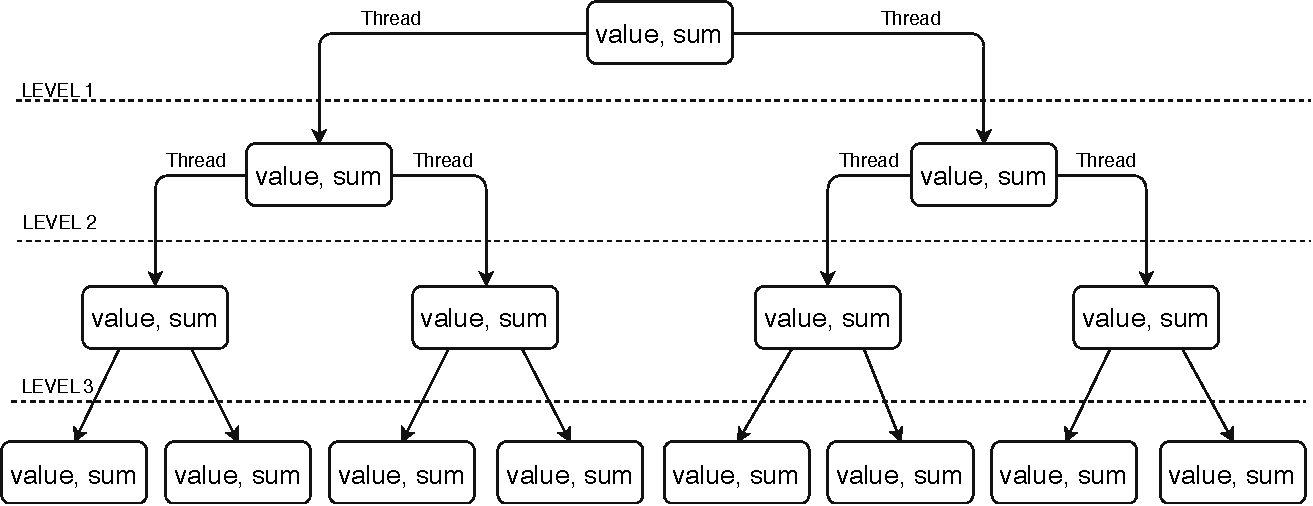
\includegraphics[width=\textwidth]{img/parallel}
	\caption{Уровни вложенности параллельной программы}
\end{figure}
Каждый вызов подсчета суммы потомоков выполняется в отдельном потоке, это происходит до дех пор, пока имеются свободные ядра процессора, после их исчерпания, подсчет выполняется последовательно.

В моем случае, на машине имеется 4 ядра, по завершению 2 уровня вложенности, будет выполняться 4 потока, и далее, для каждого из них, подсчет будет производиться последовательно.

Для синхронизации, выполнение каждого параллельного потока приостанавливается до тех пор, пока все порожденные потоки не закончат вычисления.

Исходный код приведен в листинге \ref{p1:5}.
\subsection{Параллельный алгоритм с использованием OpenMP}
Алгоритм для OpenMP аналогичен Pthreads. Благодаря использованию деректив (некоторому подобию аннотаций из Java), удалось сократить количество строк реализации.

В частности были использованы следующие дерективы:
\begin{itemize}
\item \#pragma omp parallel num\_threads(2)
\item \#pragma omp sections
\item \#pragma omp section 
\end{itemize}
Код каждой дерективы section выполняется одним потоком.

\begin{lstlisting}[firstnumber=160,language={}, caption=Отрывок TreeUtils.cpp]
unsigned long long getSumOfAllChilds_OpenMP(tnode* tree) {
    if (tree != NULL) {
        unsigned long long leftSum = 0;
	unsigned long long rightSum = 0;
		
	if (omp_get_active_level() >= omp_get_max_active_levels())
            return getSumOfAllChilds(tree);

        #pragma omp parallel num_threads(2) 
        {
            #pragma omp sections
            {
                #pragma omp section 
                { 
                    // сумма потомков для левого поддерева
                    if (tree->left != NULL){
                        tree->left->sum = getSumOfAllChilds_OpenMP(tree->left);
                        leftSum = tree->left->sum + tree->left->value;
                    }
		}

		#pragma omp section 
		{ 
                    // сумма потомков для правого поддерева
                    if (tree->right != NULL){
                        tree->right->sum = getSumOfAllChilds_OpenMP(tree->right);
                        rightSum = tree->right->sum + tree->right->value;
                    }				
		} 
            }
	}
        return leftSum + rightSum;
    }
    return 0;
}
\end{lstlisting}

\section{Тестирование}
\subsection{Эксперименты}
\subsubsection{Эксперимент 1}
\textbf{Количество потоков}: 4 (равно числу логических процессоров)\\
\textbf{Количество узлов}: от 100 до $\sim$10 000 000

\tabulinesep = 1mm
\begin{longtabu} to \textwidth {|X[ c , m ] |X[c , m ] | X[ c , m ]|X[ c , m ]|}\firsthline\hline
\textbf{Число узлов}&\textbf{Последовательный}&\textbf{OpenMP}&\textbf{Pthreads}\\ \hline \endfirsthead
100		&	\colorbox{green}{0.000002}	&	0.000816	&	0.000918\\ \hline
1000	&	\colorbox{green}{0.000019}	&	0.000545	&	0.000736\\ \hline
10000	&	\colorbox{green}{0.000368}	&	0.000654	&	0.000852\\ \hline
99932	&	0.001575	&	\colorbox{green}{0.001193}	&	0.001290\\ \hline
993761	&	0.015306	&	0.010708	&	\colorbox{green}{0.010508}\\ \hline
9486172	&	0.143309	&	\colorbox{green}{0.079550}	&	0.083088\\ \hline
\caption{Зависимость от количества узлов}
\end{longtabu}
\begin{figure}[H]
  \centering
	\fbox{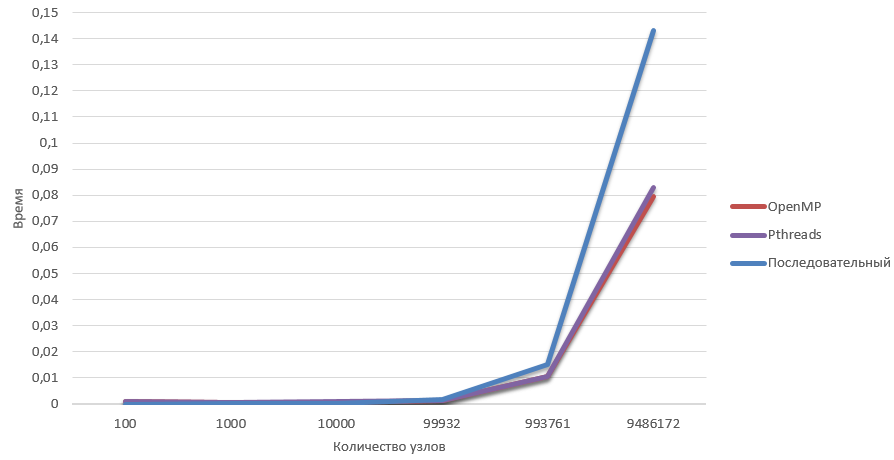
\includegraphics[width=\textwidth]{img/test1}}
	\caption{Зависимость времени от количества узлов}
\end{figure}
Из эксперимента видно, что:
\begin{itemize}
\item до 100 000 элементов, лидировало последовательное решение, после чего, уступило параллельным решениям.
\item OpenMP и Pthreads в целом показывали похожие результаты.
\end{itemize}
Для более точных результатов, необходимо провести большее числов экспериментов.
\subsubsection{Эксперимент 2}
\textbf{Количество потоков}: от 4 до 100\\
\textbf{Количество узлов}: $\sim$10 000 000

\tabulinesep = 1mm
\begin{longtabu} to \textwidth {|X[ c , m ] |X[c , m ] | X[ c , m ]|X[ c , m ]|}\firsthline\hline
\textbf{Число потоков}&\textbf{Последовательный}&\textbf{OpenMP}&\textbf{Pthreads}\\ \hline \endfirsthead
1	&	0.143858	&	\colorbox{green}{0.135808}	&	0.139525\\ \hline
2	&	-	&	0.101601	&	\colorbox{green}{0.099593}\\ \hline
4	&	-	&	\colorbox{green}{0.058160}	&	0.059163\\ \hline
6	&	-	&	\colorbox{green}{0.059542}	&	0.065316\\ \hline
8	&	-	&	0.056849	&	\colorbox{green}{0.055439}\\ \hline
12	&	-	&	0.054794	&	\colorbox{green}{0.054404}\\ \hline
16	&	-	&	\colorbox{green}{0.048021}	&	0.052502\\ \hline
20	&	-	&	\colorbox{green}{0.045488}	&	0.051346\\ \hline
32	&	-	&	0.055369	&	\colorbox{green}{0.050358}\\ \hline
50	&	-	&	0.055524	&	\colorbox{green}{0.054464}\\ \hline
80	&	-	&	0.054730	&	\colorbox{green}{0.050457}\\ \hline
100	&	-	&	\colorbox{green}{0.053519}	&	0.055099\\ \hline
\caption{Зависимость от количества потоков}
\end{longtabu}
Наилучшие показатели были получены при 16 и 20 потоках. 

При 16 потоках, прирост производительности составил:
\begin{itemize}
\item 67\% - OpenMP;
\item 64\% - Pthreads.
\end{itemize}

При 20 потоках, прирост производительности составил:
\begin{itemize}
\item 68\% - OpenMP;
\item 64\% - Pthreads.
\end{itemize}

\begin{figure}[H]
  \centering
	\fbox{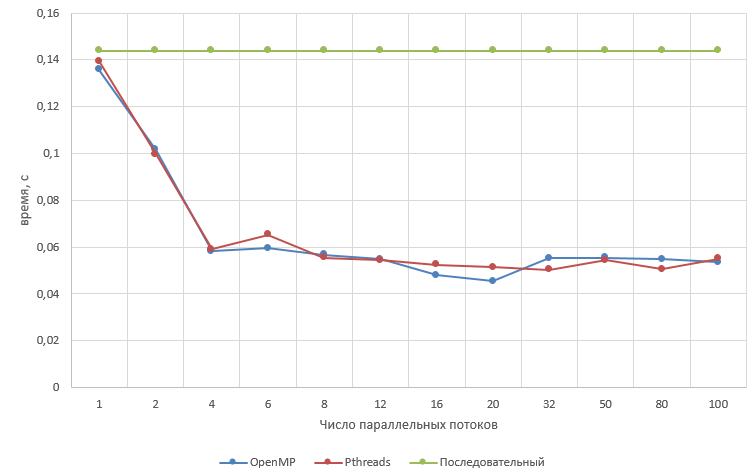
\includegraphics[width=\textwidth]{img/test2}}
	\caption{Зависимость от числа выделенных потоков}
\end{figure}

\subsubsection{Эксперимент 3}
\textbf{Количество потоков}: 20\\
\textbf{Количество узлов}: $\sim$10 000 000\\\\
В данном эксперименте проводится многократный запуск при одних и тех же характеристиках, для того чтобы вычислить:
\begin{itemize}
\item математическое ожидание;
\item дисперсию;
\item доверительный интервал для оценки среднего.
\end{itemize}
Что позволит более объективно оценить результаты алгоритмов.

\tabulinesep = 1mm
\begin{longtabu} to \textwidth {|X[c , m ] | X[ c , m ]|X[ c , m ]|}\firsthline\hline
\textbf{Последовательный}&\textbf{OpenMP}&\textbf{Pthreads}\\ \hline \endfirsthead
0.137561	&	0.060061	&	0.054078\\ \hline
0.145025	&	0.059195	&	0.062078\\ \hline
0.125417	&	0.056599	&	0.061191\\ \hline
0.125292	&	0.052370	&	0.050059\\ \hline
0.125991	&	0.062664	&	0.054928\\ \hline
0.124468	&	0.063160	&	0.056934\\ \hline
0.126880	&	0.056418	&	0.049538\\ \hline
0.126643	&	0.059022	&	0.054152\\ \hline
0.148706	&	0.053417	&	0.050933\\ \hline
0.127368	&	0.053595	&	0.054733\\ \hline
\caption{Тестовая выборка для анализа}
\end{longtabu}

\begin{longtabu} to \textwidth {|X[c , m ] |X[c , m ] | X[ c , m ]|X[ c , m ]|}\firsthline\hline
\textbf{Характеристика}&\textbf{Последовательный}&\textbf{OpenMP}&\textbf{Pthreads}\\ \hline \endfirsthead
Среднее значение				&0.1313351	&	0.0576501	&	0.0548624\\ \hline
Дисперсия						&3,89155E-06&	1,22757E-07	&	4,45013E-06\\ \hline
Доверительный интервал (P = 0.95)&[0,125742485 - 0,131245679]	&	[0,05529049 - 0,057612372]	&	[0,05221334 - 0,054820044]\\ \hline

\caption{Вероятностные характеристики}
\end{longtabu}
Как видно из представленных характеристик, \textbf{pthreads} является лучшим решением. Хоть у него и высокая дисперсия, средняя скорость вычисления используя его выше чем у OpenMP.




\clearpage
\addcontentsline{toc}{section}{Вывод}
\section*{Вывод}
В данной работе были рассмотрены методы распараллеливания программ с использованием \textbf{OpenMP} и \textbf{Pthreads}.

Реализация на OpenMP заняла меньшее количество строк кода, по сравнению с Pthreads. Например, в Pthreads необходимо использовать функцию \textbf{pthread\_join} для синхронизации потоков, в то время как в OpenMp это контроллирует сам фреймворк.

Эксперименты показали, что прирост проиводительности начался при наличии в деревее более 100 000 узлов. Наилучшие результаты были получены при 20 потоках, где удалось добиться прироста производительность в 68\% для OpenMP и 64\% для Pthreads. Само вычисление было выполнено в 3.2 раза быстре последовательного решения. Возможно, данный показатель в 3.2 раза, можно повысить если избавиться от многих процессов, работающих в фоне.

Отсюда можно сделать вывод, что распараллеливании программ имеет смысл в трудоемких задачах, в то время как в тривиальных задачах, последовательное решение будет быстрее.


%------------------------------------------------------------------------------

%\clearpage
%\addcontentsline{toc}{section}{Список литературы}
%\bibliography{thesis}
%\bibliographystyle{ugost2008}


\clearpage
\addcontentsline{toc}{section}{Приложения}
\setcounter{section}{0}
\section*{Приложение 1} 
\lstinputlisting[caption=Main.cpp, label=p1:1]{sourceCode/Main.cpp}
\section*{Приложение 2}
\lstinputlisting[caption=Tree.h, label=p1:2]{sourceCode/Tree.h}
\section*{Приложение 3}
\lstinputlisting[caption=Tree.cpp, label=p1:3]{sourceCode/Tree.cpp}
\section*{Приложение 4}
\lstinputlisting[caption=TreeUtils.h, label=p1:4]{sourceCode/TreeUtils.h}
\section*{Приложение 5}
\lstinputlisting[caption=TreeUtils.cpp, label=p1:5]{sourceCode/TreeUtils.cpp}




%\nocite{anatomy}
\end{document}
